\clearpage
\slidetitle{Reconnaissance}

\begin{slide}

\begin{itemize}

	\item On choisit une association entre vecteur de sortie dans $\mathbb{R}^q$ et caractères à reconnaître:

	\begin{equation*}
		\begin{pmatrix}
			1 \\ 0 \\ 0 \\ \vdots \\ 0
		\end{pmatrix}
		\mapsto \text{"A"}
		\qquad
		\begin{pmatrix}
			0 \\ 1 \\ 0 \\ \vdots \\ 0
		\end{pmatrix}
		\mapsto \text{"B"}.
	\end{equation*}


	\item Si les poids sont adaptés, le principe de reconnaissance est simple.

% 	\item Calcul récursif de l'image \texttt{sorties[-1]} du \texttt{Reseau}.

% \begin{lstlisting}[language=Python]
% def sortie(self, vecteur):
% 	sorties = [vecteur + [-1]]
% 	taille = len(self)
% 	for couche in self:
% 		sortie = [neurone.sortie(sorties[-1]) for neurone in couche] 
% 		if len(sorties) < taille:
% 			sortie += [-1]
% 		sorties.append(sortie)
% 	return sorties
% \end{lstlisting}

\end{itemize}

\begin{figure}[!h]

	\centering

	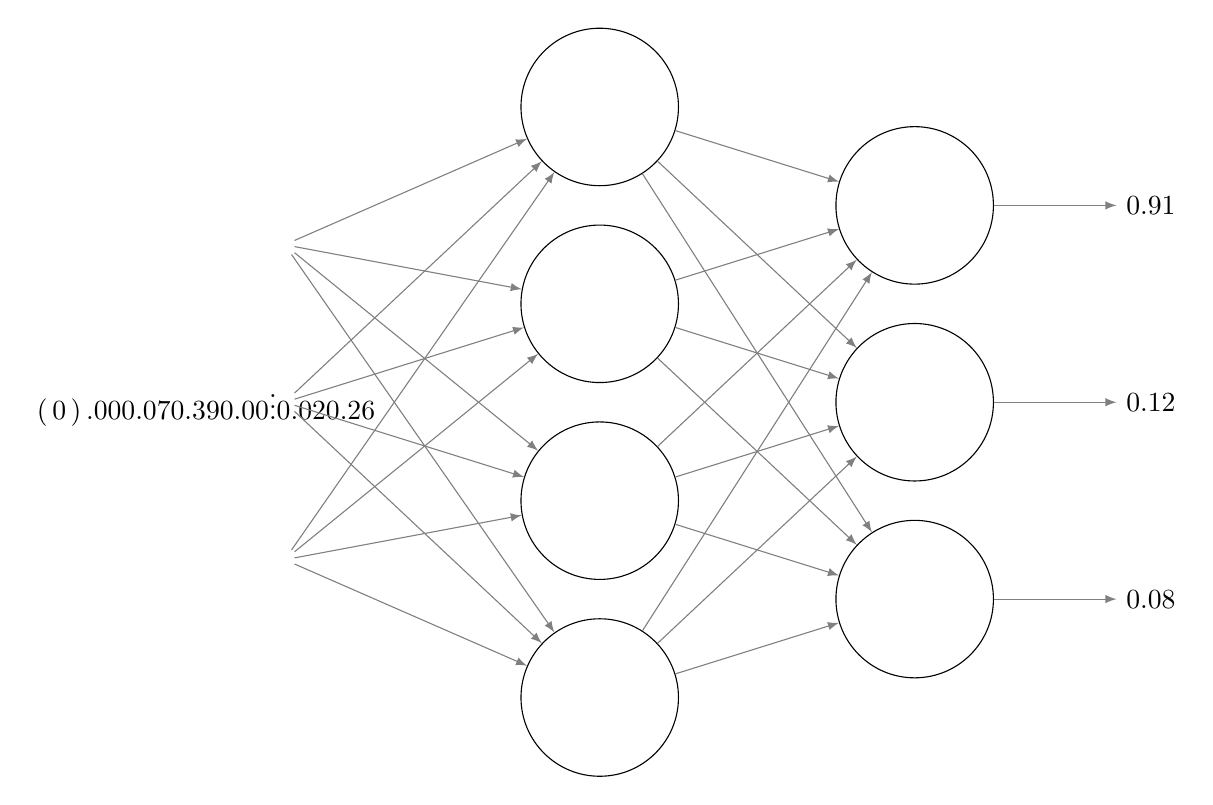
\begin{tikzpicture}[scale=1, x=1cm, y=1cm]

		\tikzstyle{neurone}=[draw, transform shape, circle, minimum size=2cm]
		\tikzstyle{entree}=[draw, transform shape, rectangle, minimum size=1.5cm]
		\tikzstyle{fleche}=[->, >=latex, gray]

		\node at (-1, 0) {
		$\begin{pmatrix}
			0.00 \\ 0.07 \\ 0.39 \\ 0.00 \\ \vdots \\ 0.02 \\ 0.26
		\end{pmatrix}$
		};

		\node (e1) at (0, -2) {};
		\node (e2) at (0, 0) {};
		\node (e3) at (0, 2) {};

		\node[neurone] (n11) at (4, 3.75) {};
		\node[neurone] (n12) at (4, 1.25) {};
		\node[neurone] (n13) at (4, -1.25) {};
		\node[neurone] (n14) at (4, -3.75) {};

		\node[neurone] (n21) at (8, 2.5) {};
		\node[neurone] (n22) at (8, 0) {};
		\node[neurone] (n23) at (8, -2.5) {};

		\draw[fleche] (e1) -- (n11);
		\draw[fleche] (e1) -- (n12);
		\draw[fleche] (e1) -- (n13);
		\draw[fleche] (e1) -- (n14);
		\draw[fleche] (e2) -- (n11);
		\draw[fleche] (e2) -- (n12);
		\draw[fleche] (e2) -- (n13);
		\draw[fleche] (e2) -- (n14);
		\draw[fleche] (e3) -- (n11);
		\draw[fleche] (e3) -- (n12);
		\draw[fleche] (e3) -- (n13);
		\draw[fleche] (e3) -- (n14);

		\draw[fleche] (n11) -- (n21);
		\draw[fleche] (n11) -- (n22);
		\draw[fleche] (n11) -- (n23);
		\draw[fleche] (n12) -- (n21);
		\draw[fleche] (n12) -- (n22);
		\draw[fleche] (n12) -- (n23);
		\draw[fleche] (n13) -- (n21);
		\draw[fleche] (n13) -- (n22);
		\draw[fleche] (n13) -- (n23);
		\draw[fleche] (n14) -- (n21);
		\draw[fleche] (n14) -- (n22);
		\draw[fleche] (n14) -- (n23);

		\node (s1) at (11, 2.5) {$0.91$};
		\node (s2) at (11, 0) {$0.12$};
		\node (s3) at (11, -2.5) {$0.08$};

		\draw[fleche] (n21) -- (s1);
		\draw[fleche] (n22) -- (s2);
		\draw[fleche] (n23) -- (s3);

		% \draw[thick, decoration={brace, amplitude=0.3cm}, decorate] (s1.north east) -- (s3.south east);
		% \node[align=left, xshift=2.5cm] at (s2.east) {comparaison\\ aux vecteurs\\ choisis};

	\end{tikzpicture}

\end{figure}

\end{slide}